\documentclass[12pt]{extarticle}
\usepackage{tempora}
\usepackage[T1, T2A]{fontenc}
\usepackage[utf8]{inputenc}
\usepackage[english, ukrainian]{babel}
\usepackage{geometry}
\usepackage{graphicx}
\usepackage{multirow}
\usepackage{multicol}
\usepackage{float}
\usepackage{indentfirst}
\graphicspath{{/home/artem/Pictures}}
\geometry
{
    a4paper,
    left=30mm,
    top=15mm,
    right=20mm,
    bottom=15mm,
}

\begin{document}
\begin{titlepage}
    \begin{center}
        \textbf{\normalsize{\MakeUppercase{
            Міністерство Освіти і науки України
            Національний університет "Львівська політехніка"
        }}}

        \begin{flushright}
        \textbf{ІКНІ}\\
        Кафедра \textbf{ПЗ}
        \end{flushright}
        \vspace{15mm}

        \includegraphics[width=0.4\textwidth]{lpnu_logo.png}

        \vspace*{\fill}

        \textbf{\normalsize{\MakeUppercase{Звіт}}}
            
        До лабораторної роботи №14

        \textbf{на тему:} “Дослідження роботи web-сервера та протоколу HTTP.”

        \textbf{з дисципліни:} “Організація комп'ютерних мереж”
            
        \vspace*{\fill}

        \begin{flushright}

            \textbf{Лектор:}\\
            доцент кафедри ПЗ\\
            Крук О.Г.\\
            \vspace{12pt}

            \textbf{Виконав:}\\
            студент групи ПЗ-24\\
            Губик А. С.\\
            \vspace{12pt}

            \textbf{Прийняв:}\\
            доцент кафедри ПЗ\\
            Задорожний І. М.\\
        \vspace{12pt}
        \end{flushright}

        Львів -- 2023
            
            
    \end{center}
\end{titlepage}

\textbf{Тема роботи:} Дослідження роботи web-сервера та протоколу HTTP.
\vspace{12pt}

\textbf{Мета роботи:} Ознайомитися основами протоколу HTTP, дослідити формат
повідомлень HTTP.

\textbf{Теоритичні відомості:}
HTTP (Hyper Text Transfer Protocol - протокол передачі гіпертекстових
документів) – протокол прикладного рівня, основним призначенням якого є
передача веб-сторінок (текстових файлів з розміткою HTML).
HTTP є клієнт-серверним протоколом. Робота по протоколу HTTP
відбувається наступним чином: програма-клієнт встановлює TCP-з'єднання з
сервером (стандартний номер порту-80) і видає йому HTTP-запит. Сервер
обробляє цей запит і видає HTTP-відповідь клієнту. Cервер (веб-сервер)
обслуговує запити клієнтів (наприклад, повертає запитувану клієнтом
сторінку).
Клієнт звертається з запитами до сервера. Основні реалізації клієнта – це
браузери. Окрім клієнта та сервера, визначена ще одна роль – проксі. Проксі –
це проміжна програма, яка виконує функції як сервера, так і клієнта. Проксі
обслуговує запит так, як би це робив первинний сервер. Запити можуть
обслуговуватися всередині проксі або ж переадресовуватися іншим серверам.
Обмін даними в HTTP відбувається за схемою “запит–відповідь”. Важливою
рисою HTTP є те, що цей протокол не зберігає стану.
\break
\subsection*{Хід роботи}



\begin{figure}[H]
    \centering
    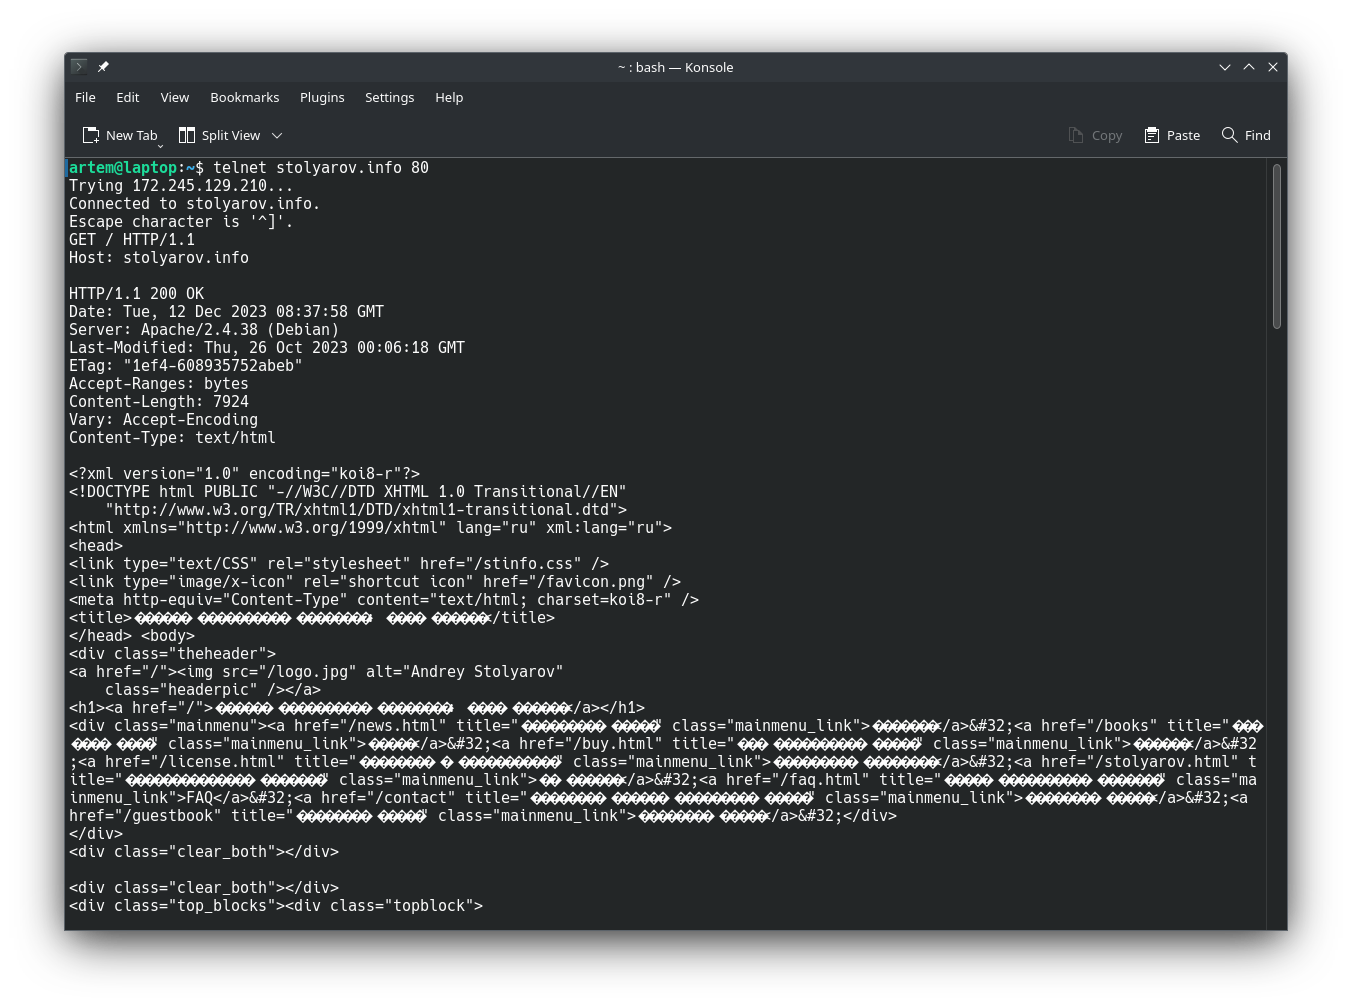
\includegraphics[width=0.90\textwidth]{GET}
    \caption{}
\end{figure}

\begin{figure}[H]
    \centering
    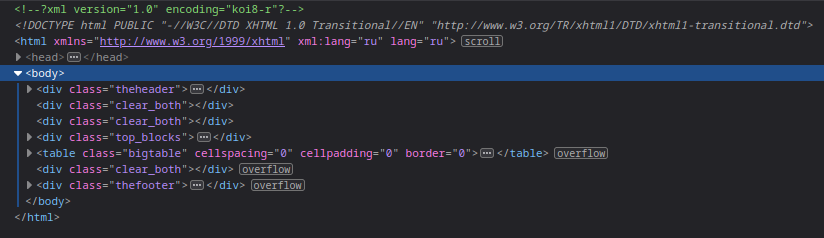
\includegraphics[width=0.90\textwidth]{firefox}
    \caption{}
\end{figure}

\begin{figure}[H]
    \centering
    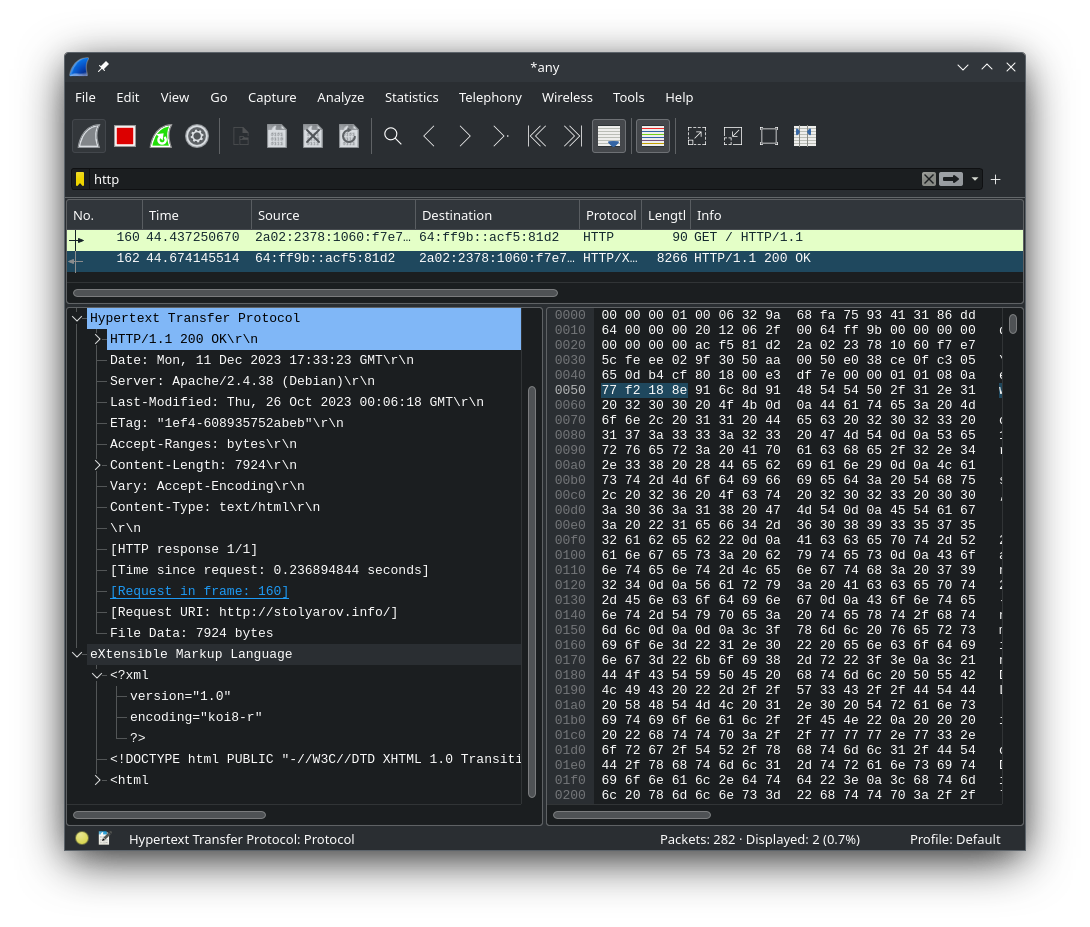
\includegraphics[width=0.90\textwidth]{wireshark}
    \caption{}
\end{figure}

\begin{figure}[H]
    \centering
    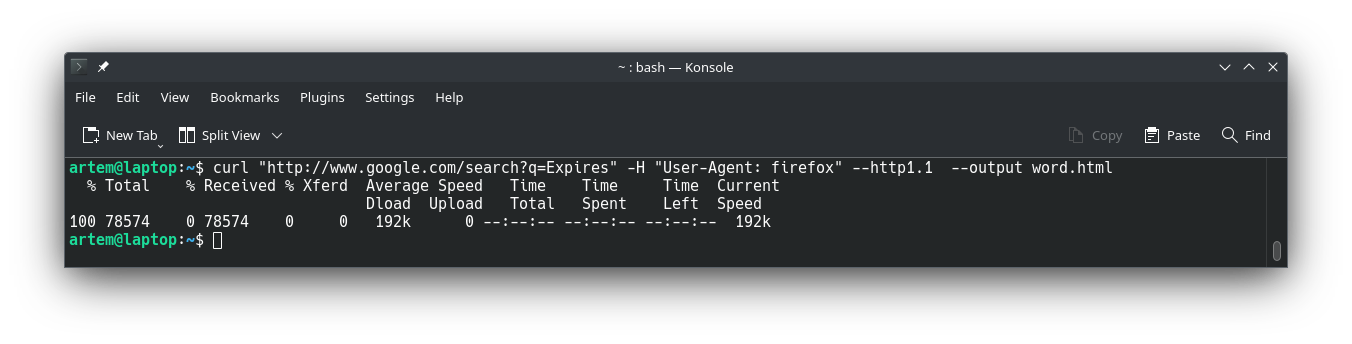
\includegraphics[width=0.90\textwidth]{curl_expires}
    \caption{}
\end{figure}

\begin{figure}[H]
    \centering
    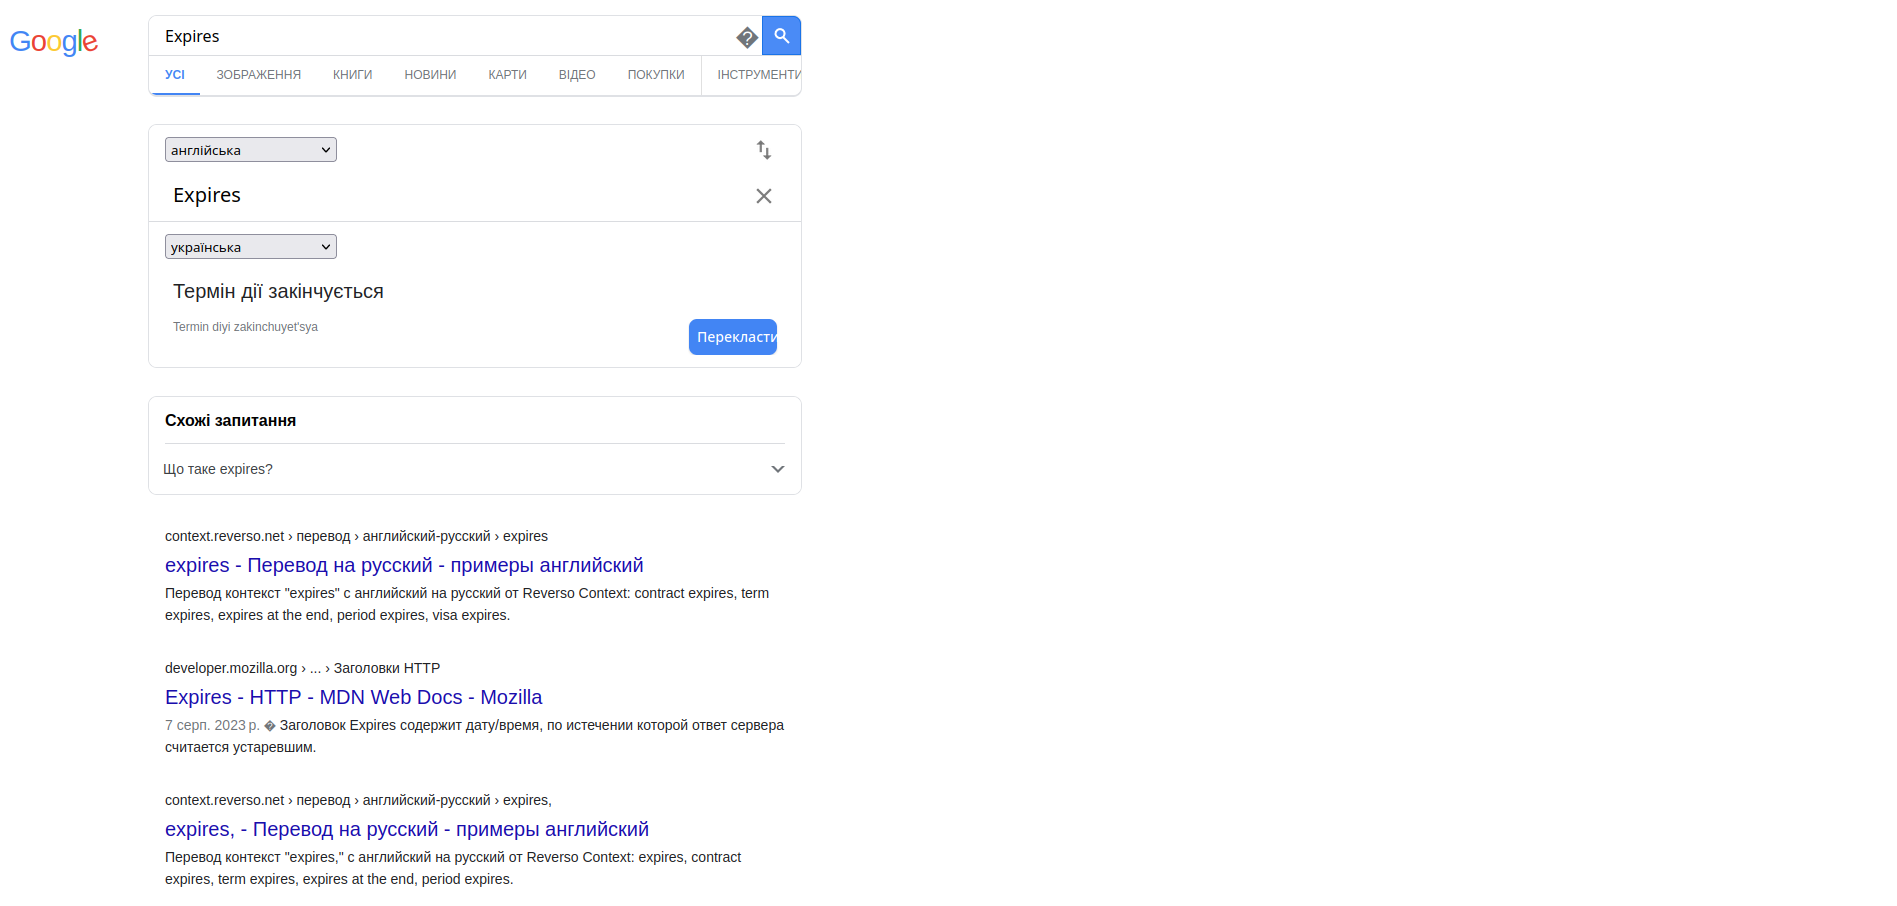
\includegraphics[width=0.90\textwidth]{expires}
    \caption{}
\end{figure}

\begin{figure}[H]
    \centering
    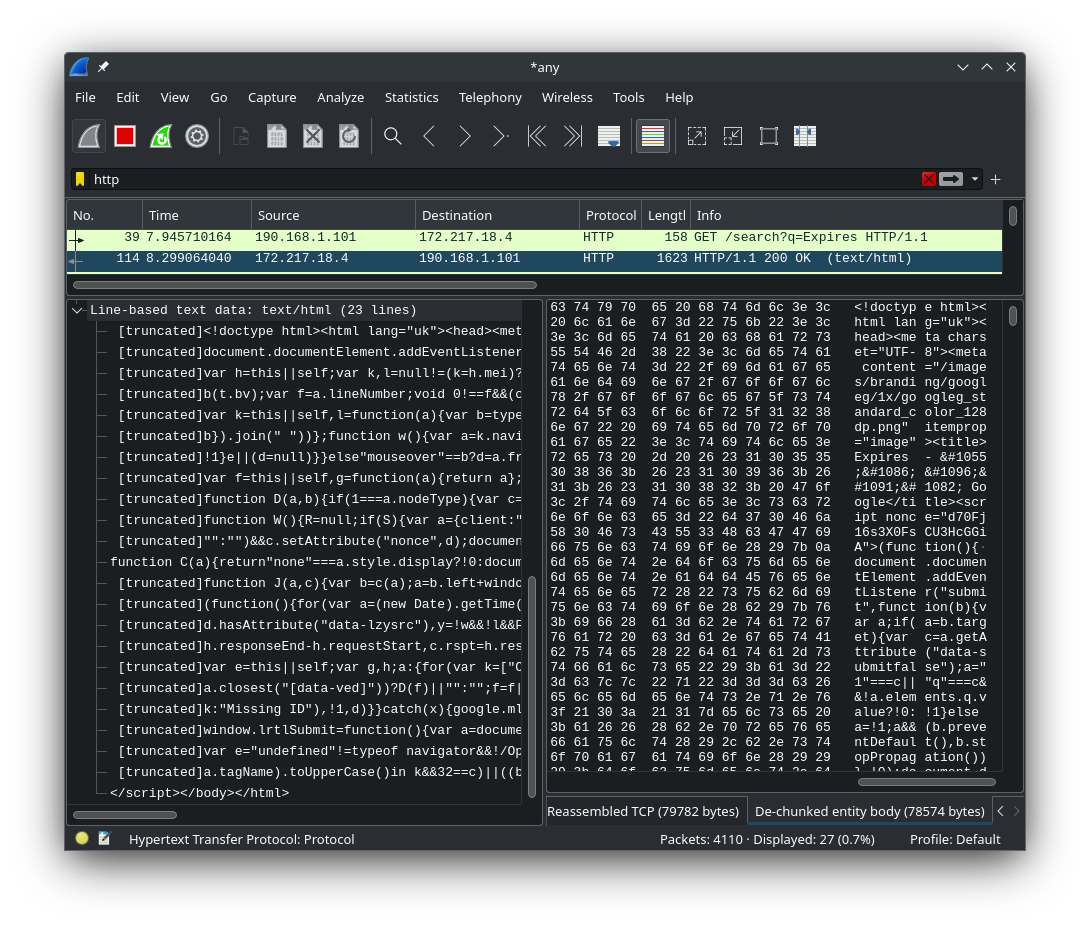
\includegraphics[width=0.90\textwidth]{shark_expires}
    \caption{}
\end{figure}
\begin{figure}[H]
    \centering
    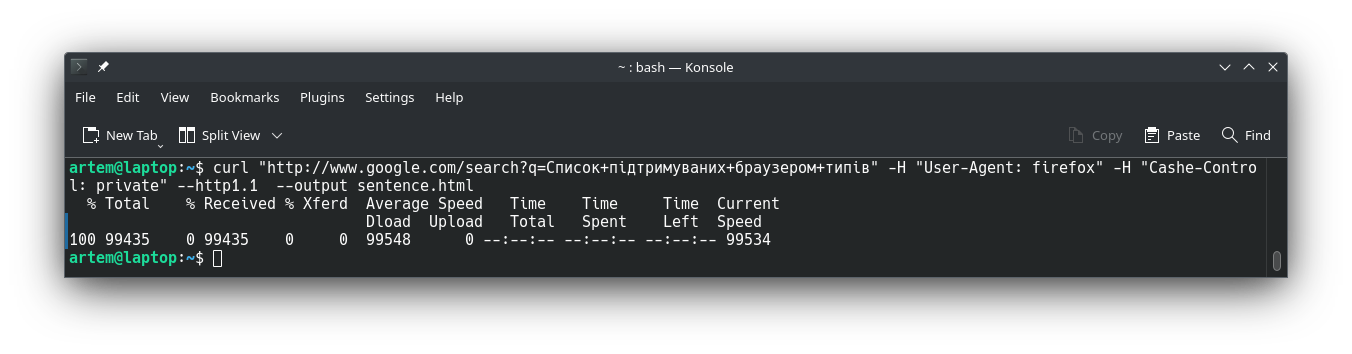
\includegraphics[width=0.90\textwidth]{private}
    \caption{}
\end{figure}
\begin{figure}[H]
    \centering
    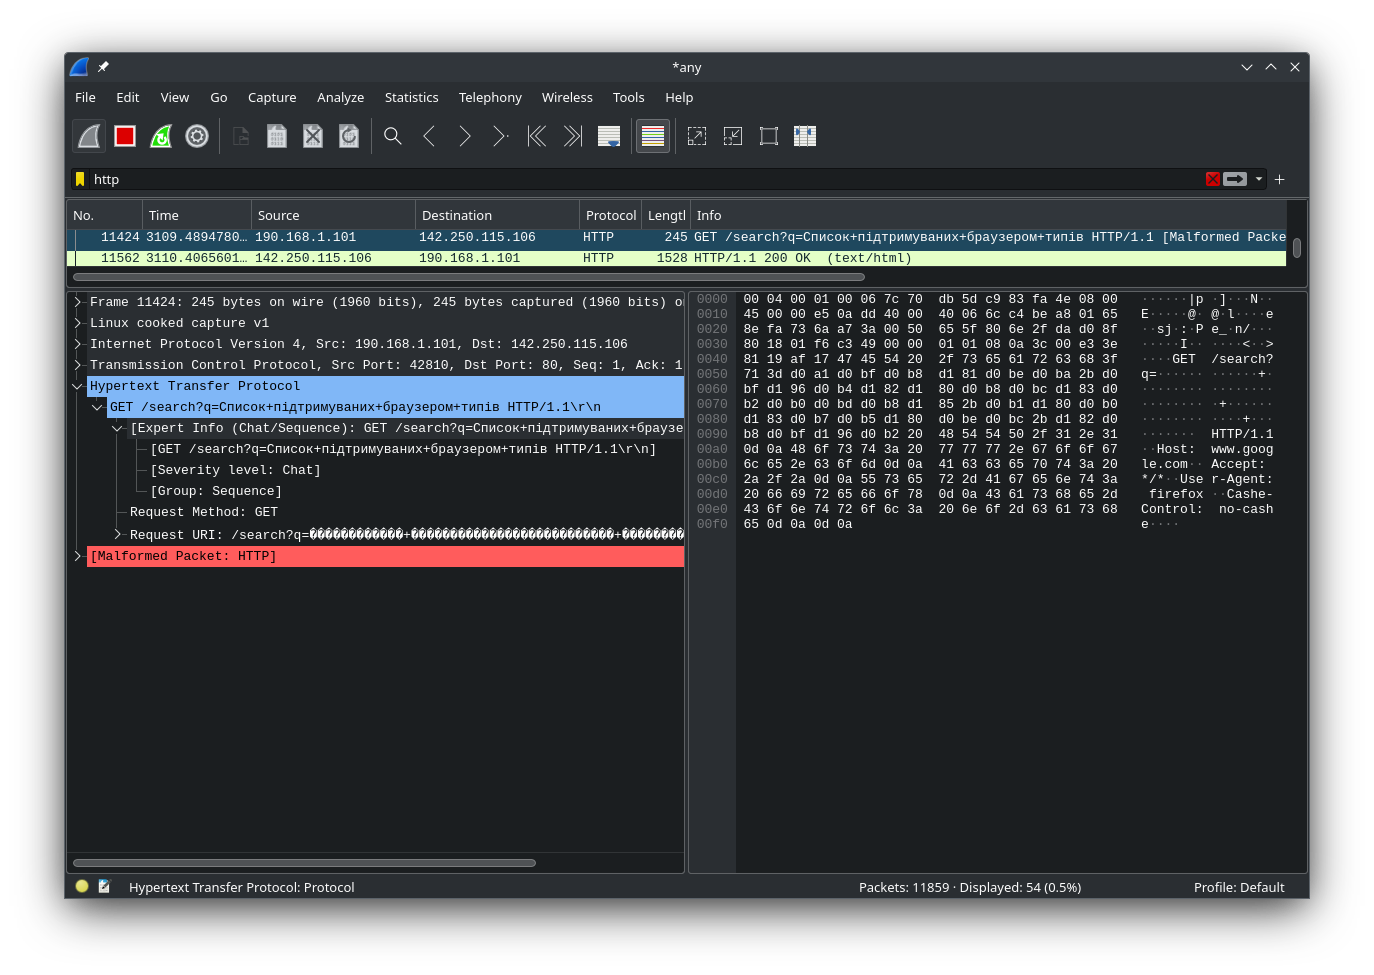
\includegraphics[width=0.90\textwidth]{shark_no_cashe}
    \caption{}
\end{figure}
\begin{figure}[H]
    \centering
    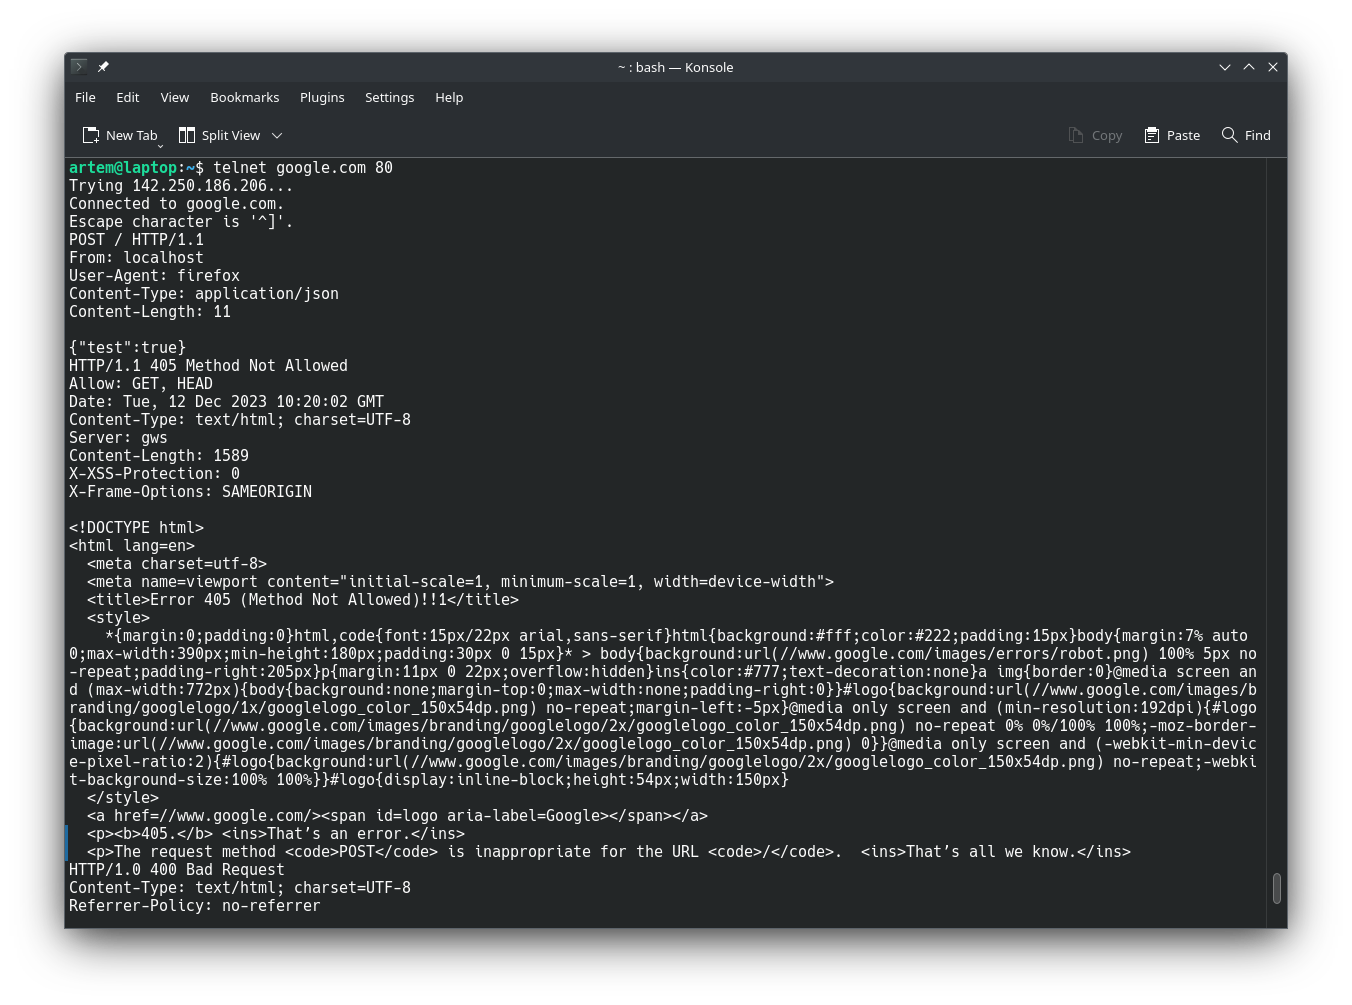
\includegraphics[width=0.90\textwidth]{post}
    \caption{}
\end{figure}
\begin{figure}[H]
    \centering
    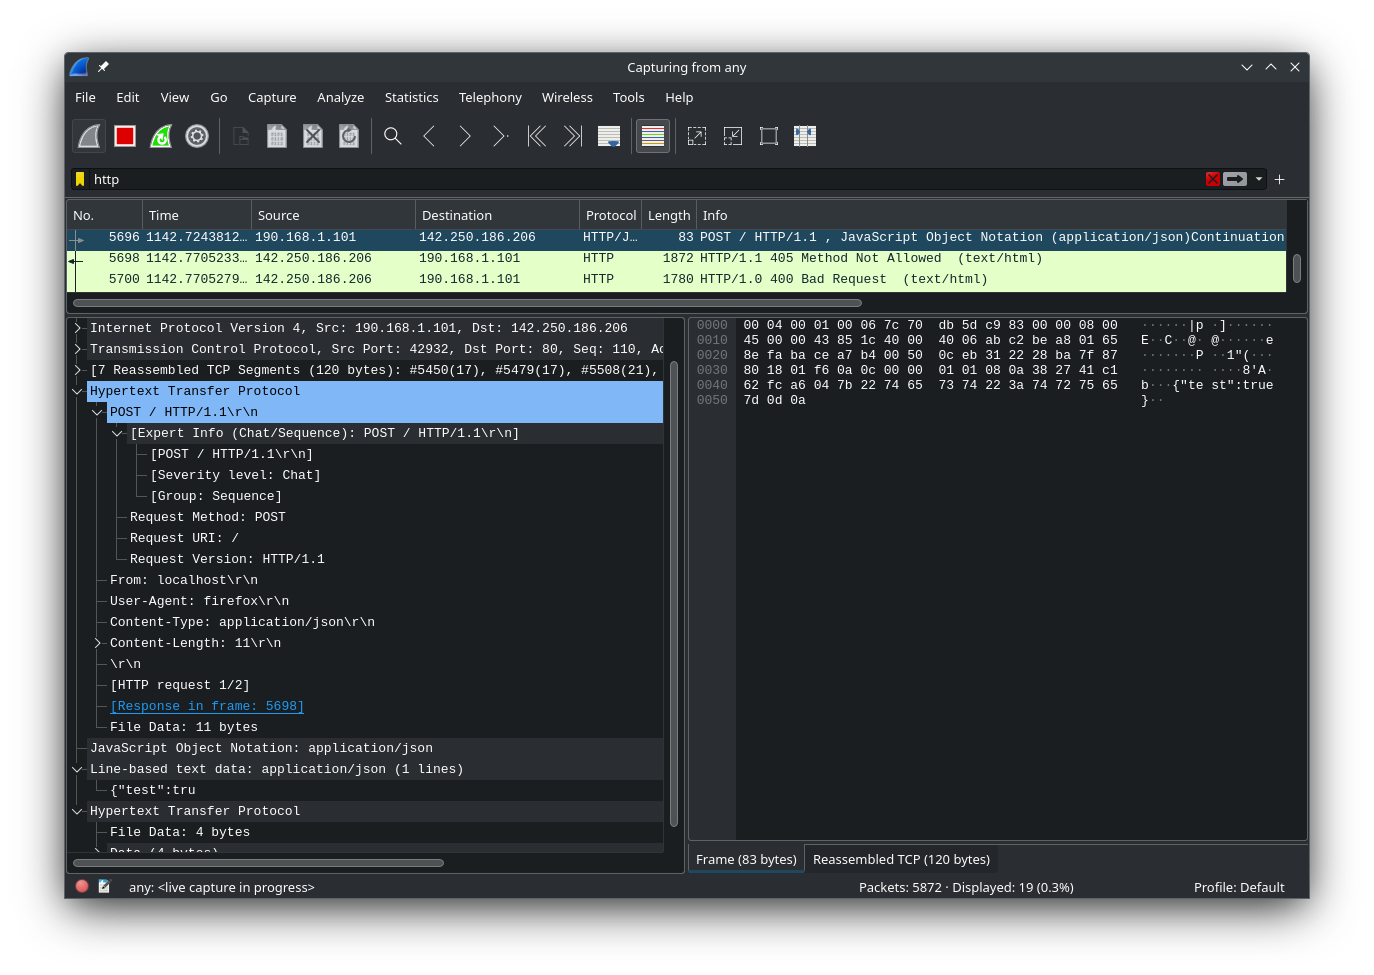
\includegraphics[width=0.90\textwidth]{shark_post}
    \caption{}
\end{figure}



\subsection*{Висновок} 
Освоїв роботу з HTTP протоколом. 
\end{document}